\begin{figure*}[htbp] \centering
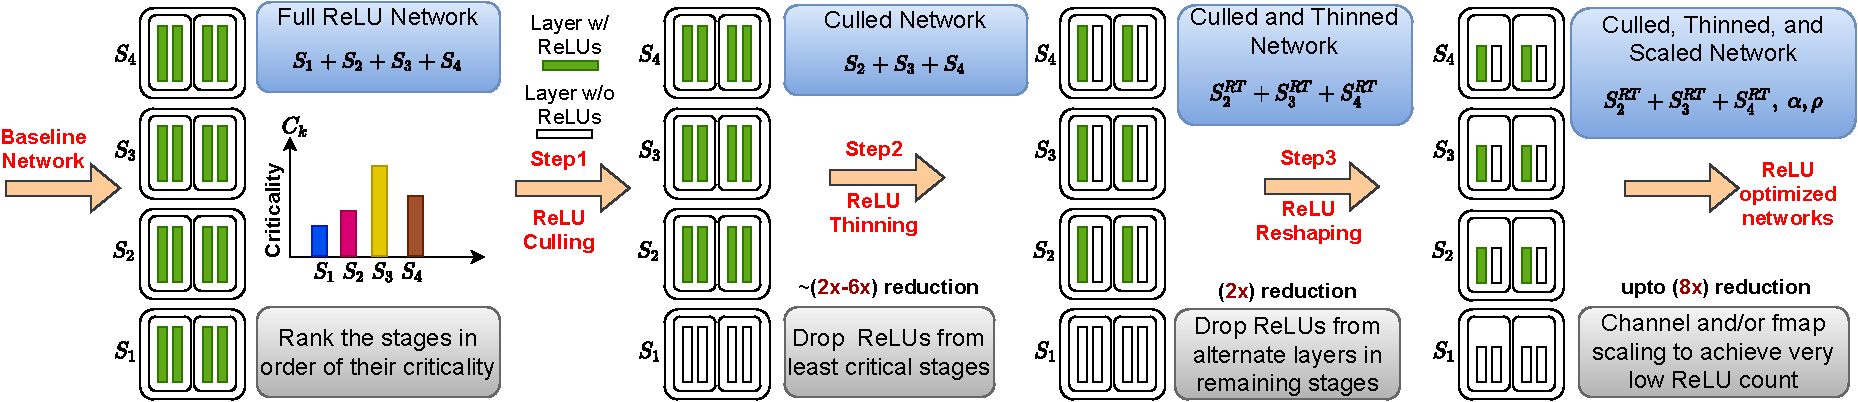
\includegraphics[scale=0.55]{Figures/2020_ReluDropout}
\caption{The DeepReDuce ReLU optimization pipeline.
The baseline is optimized left to right following orange arrows.
Green (plain) boxes indicate layer's with (without) ReLUs, gray boxes indicate profiling steps to guide optimizations, and blue boxes describe the resulting network after each optimization step. Given a baseline network, DeepReDuce outputs ReLU-optimized networks preserving as much accuracy from the baseline network
as possible.}
\label{fig:BlockDiagramDeepReDuce}
\end{figure*}

\section{DeepReDuce} 
\label{sec:Method}

Using the insights listed above, this section presents the proposed ReLU optimizations and
resulting method for optimizing networks for private inference.
Given a baseline network as input,
DeepReDuce outputs a set of Pareto optimal networks 
that trade accuracy and ReLU count.
This is done via three ReLU reducing optimizations 
(shown as Step 1 to 3 in Figure \ref{fig:BlockDiagramDeepReDuce}):
Culling (Section \ref{sec:culling}), Thinning  (Section~\ref{sec:Thinning}), and Reshaping (Section~\ref{sec:Reshaping}). 
The optimizations work at different levels of granularity and are applied sequentially
to identify high-performing networks quickly.


\subsection{ReLU Culling}
\label{sec:culling}

The first optimization, named \textit{ReLU Culling}, 
removes ReLUs at a coarse granularity (Step 1 in Figure \ref{fig:BlockDiagramDeepReDuce}).
It works by completely removing all ReLUs from a given network stage.
Culling is applied iteratively,
from least to most critical using a criticality metric (described below)
that estimates the importance of each stage's ReLUs.  
Empirically we find the initial stage tends to be highly amenable to Culling as it 
contains a large number of non-critical ReLUs.
For a network with $D$ stages, ReLU Culling outputs $D-1$ networks that trade accuracy for reduced ReLU counts.

{\bf Criticality metric:} 
The order that a network's stages are culled is determined by estimating ReLU criticality,
i.e., how important a particular stage's ReLUs are for accuracy.
We denote each stage's ($S_k$) criticality as $C_k$.
To determine criticality, we first remove all the ReLUs from all network stages except $S_k$,
train the network, measure its accuracy, and then repeat the process with KD using the original network as a teacher. 
The criticality metric $C_k$ captures the accuracy improvement from retaining ReLUs in stage $S_k$ and the stage's ReLU cost as follows:

\begin{equation} \label{eqn:CriticalityMetric}
C_k = \frac{Acc [S_k] - \min_{(i=1 \; to \; D)} \{ Acc[Si] \}}{(\#ReLU [S_k])^{w}}  
\end{equation}

In Equation~\ref{eqn:CriticalityMetric}, $Acc [S_k]$ is the accuracy of the network with ReLUs only in stage $S_k$ trained with KD. 
$\#ReLU [S_k]$ in the denominator is the number of ReLUs in stage $S_k$. 
The hyper-parameter $w$ controls the weighted importance of accuracy and ReLU count, 
we set $w$=0.07, similar to \cite{tan2019efficientnet}.
The value of $C_k$ corresponding to least critical stage would be zero (see Table \ref{tab:ResNetBlockDropout}) and stages with higher $C_k$ utilize ReLUs better than stages with lower $C_k$. Hence, they are more critical and dropped later in DeepReDuce. We note that, even for the same network, criticality of ReLUs varies across different datasets. For instance, as shown in Table \ref{tab:ResNetBlockDropout} the criticality order of ResNet18 on CIFAR-100, from least to most critical, is $S_1 < S_4 < S_2 < S_3$ (calculated from the Table \ref{tab:ReluHeteroR18}); whereas, the same on TinyImageNet is $S_1 < S_2 < S_4 < S_3$. 


\subsection{ReLU Thinning}
\label{sec:Thinning}
To further reduce ReLU counts, each Culled network from the ReLU Culling stage is further Thinned 
by dropping alternate ReLU layers in the remaining non-Culled stages of the network 
(Step 2 in Figure \ref{fig:BlockDiagramDeepReDuce}). This yields an additional reduction in ReLU counts for each Culled networks as the number of ReLU layers are halved.
%reduced by $2\times$. 


%\textcolor{red}{when layers in non-Culled Stages are symmetrical and having equal \#ReLUs (e.g., ResNet18). However, when alternate layers are asymmetrical and have unequal \#ReLUs, the reduction in ReLU count depends on the layers which have following ReLUs (e.g., MobileNetV1 \cite{howard2017mobilenets}). The detailed discussion is included in the Appendix \ref{SecAppendix:ParetoPointsMV1}.} 
  
Note that the same reduction in ReLU counts can be achieved via other means, for example, 
by dropping ReLUs from the first half or last half of a stage, or  
by scaling the number of channels in each 
layer by $2\times$. 
However, we empirically find that ReLU Thinning consistently outperforms both 
approaches (see results in Section~\ref{sec:Motivation}). 
Moreover, our empirical findings resonate with the observations made in~\cite{zhao2018reThinking}, which claims that removing ReLUs from alternate layers regularize the network and prevent information loss.

While Thinning could be generalized to drop ReLUs from arbitrary layers in non-Culled stages, this would significantly increase search complexity. Our choice of dropping ReLUs from alternate layers in non-Culled stages is to strike a balance between run-time and effectiveness of DeepReDuce.




\begin{table} [t] \centering
\caption{ReLUs' Criticality on TinyImageNet for ResNet18/34. FR is baseline with Full-ReLU ($S_1$+$S_2$+$S_3$+$S_4$). Similar to the our observations on CIFAR-100 in Table \ref{tab:ReluHeteroR18}, accuracy differs significantly across stages and $S_1$ ($S_3$) ReLUs are least (most) critical.}
\label{tab:ResNetBlockDropout} 
\resizebox{.49\textwidth}{!}{
\begin{tabular}{ccccccccc} \toprule
\multirow{2}{*}{ Net } & \multicolumn{4}{c}{ ResNet18 } & \multicolumn{4}{c}{ ResNet34 } \\ 
\cmidrule(lr{0.5em}){2-5}  
\cmidrule(lr{0.5em}){6-9} 
& \#ReLUs & W/o KD(\%) & W/ KD(\%) & $C_k$ &\#ReLUs & W/o KD(\%) & W/ KD(\%) & $C_k$ \\ \toprule
FR & 2228K & 61.28 & - &    -   &3867K & 63.06 & -     &  - \\ 
$S_1$ & 1049K & 41.90 & 39.61 &  0.00  &1573K & 42.10 & 39.4 & 0.00\\
$S_2$ & 524K & 50.53 & 49.44 & 6.04   &1049K & 53.49 & 51.74 & 7.58\\
$S_3$ & 262K & 51.93 & 54.34 &  9.50  &786K & 57.28 & 60.83 & 13.44 \\
$S_4$ & 131K & 46.89 & 51.46 &  8.02  &197K & 48.10 & 54.41 & 10.37 \\ \bottomrule
\end{tabular} }
\end{table}








% & stages & \#ReLUs & w/o KD & w/ KD \\ \toprule
%\multirow{9}{*}{ \rotatebox[origin=c]{90}{ResNet18} } &$S_1$ + $S_2$ + $S_3$ + $S_4$ & 2228K & 61.28 & - \\ \cline{2-5}
%& $S_1$ + $S_2$ + $S_3$& 1836K & 58.92 & 60.78 \\
%& $S_1$ + $S_2$ + $S_4$ & 1704K & 59.42 & 62.98 \\
%& $S_1$ + $S_3$ + $S_3$ & 1442K & 60.12 & 64.45 \\
%& $S_2$ + $S_3$ + $S_4$ & 918K & 60.5 & 64.66 \\  \cline{2-5}
%& $S_1$ & 1049K & 41.9 & 39.61 \\
%& $S_2$ & 524K & 50.53 & 49.44 \\
%& $S_3$ & 262K & 51.93 & 54.34 \\
%& $S_4$ & 131K & 46.89 & 51.46 \\ \midrule
%\multirow{9}{*}{ \rotatebox[origin=c]{90}{ResNet34} } & $S_1$ + $S_2$ + $S_3$ + $S_4$ & 3867K & 63.06 & - \\  \cline{2-5}
%& $S_1$ + $S_2$ + $S_3$ & 3408K & 61.93 & 65.01 \\
%& $S_1$ + $S_2$ + $S_4$ & 2818K & 61.19 & 64.73 \\
%& $S_1$ + $S_3$ + $S_3$ & 2556K & 62.2 & 65.92 \\
%& $S_2$ + $S_3$ + $S_4$ & 2032K & 63.45 & 66.69 \\  \cline{2-5}
%& $S_1$ & 1573K & 42.1 & 39.4 \\
%& $S_2$ & 1049K & 53.49 & 51.74 \\
%& $S_3$ & 786K & 57.28 & 60.83 \\
%& $S_4$ & 197K & 48.1 & 54.41 \\

\subsection{ReLU Reshaping}
\label{sec:Reshaping}
The final optimization of DeepReDuce uses conventional channel and fmaps resolution scaling
to decrease ReLU counts by reducing network size and shape 
(Step 3 in Figure \ref{fig:BlockDiagramDeepReDuce}).
While less effective than Culling and Thinning, as they tend to introduce higher accuracy drop, 
these optimization are useful in producing networks for highly-constrained ReLU budgets. 

To down-scale networks we explore three alternatives: 
channel scaling, feature map (fmap) scaling, and compound scaling.
Channel and fmap-resolution scaling reduce the filter count and spatial dimensions of fmaps across the network by factors of $\alpha$ and $\rho$, respectively. 
Compound scaling scales both channels and fmap spatial dimensions simultaneously, achieving multiplicative reductions in ReLU count. 
More precisely, channel and fmap resolution scaling by $\alpha$ and $\rho$ reduce the ReLU count by   $\alpha$ and $\rho^2$ respectively.
Since our aim is to gradually reduce the ReLU count, we first employ channel scaling ($\alpha$=0.5) and then fmap scaling ($\rho$=0.5) followed by compound scaling ($\alpha$=0.5 and $\rho$=0.5) to reduce the ReLU count by 2$\times$, 4$\times$, and 8$\times$, respectively. 

One can use different scaling factors for different degree of ReLU reduction.
However, naively selected scaling factors could result in suboptimal ReLU networks. 
For instance, $\alpha$=0.25 and $\rho$=0.5 both lower the ReLU count by 4$\times$; however, the former produces less accurate networks (see accuracy with KD in Table \ref{tab:AlphaVsRhoComp} in Appendix \ref{secAppendix:ChannelVsFmapScaling}). One possible explanation for the lower accuracy in channel-scaled networks can be the lower parameter count. 
That is, while $\alpha$=0.25 and $\rho$=0.5 reduces the ReLU count by same degree the former also reduces the parameter count by 4$\times$, which can reduce the expressiveness of the network.

We note that because Reshaping is
applied to all stages equally, it scales down the sizes of critical layers as well. 
As such, applying Reshaping earlier would reduce opportunities for our more effective Culling and Thinning optimizations. 
This is why we use Reshaping only as a last resort to reduce ReLU count.


\subsection{Improving accuracy using KD}
To maximize the accuracy of Culled, Thinned, and Reshaped networks we employ
knowledge distillation (KD) as the final step of DeeReDuce. 
Specifically, we re-train ReLU-optimized networks with Full-ReLU baseline  as a teacher, and
find distillation typically recovers several percentage points of accuracy on our datasets.
We note that although KD is only explicitly used as a final step, it is implicitly incorporated in the evaluation of stage criticality (see Section~\ref{sec:culling}), and guides the selection of which stages to Cull first (or last). 
Since the gain in accuracy from KD depends on the position of stages (Table \ref{tab:ReluHeteroR18} and \ref{tab:ResNetBlockDropout}), order of stage criticality computed with KD is different compared to that computed without KD. 
Therefore, incorporating KD ($Acc [S_k]$ in Eq. \ref{eqn:CriticalityMetric}) in computing criticality produces better results. 


\subsection{Putting it All Together}

We developed DeepReDuce to effectively apply the above optimizations without exhaustively exploring the design space.
Given a network as input, DeepReDuce first determines the criticality of each stage.
We use this information to guide the application of coarse-grained ReLU Culling.
DeepReDuce iteratively applies Culling to each network stage from least to most critical.
The application of Culling is compounded after each iteration,
e.g., if S$_{2}$ was Culled first and S$_{3}$ is the next least critical stage, 
then DeepReDuce Culls both S$_{2}$ and S$_{3}$ in the following iteration.

%{\bf Quantifying ReLU Reduction in Each Steps} 
%\textcolor{red}{
%The amount of ReLU reduction in each steps varies across the networks and the spatial size of input images. Nevertheless, we found that ReLU culling reduces the ReLU count by a huge margin and hence a most effective step in DeepReDuce. For example, in ResNet18 this ranges from 2.42$\times$ (when $S_1$ is culled) to 8.4$\times$ (when $S_1$, $S_2$, and $S_4$ are culled). The other steps in DeepReDuce, systematically reduces the ReLU count by to reach a target ReLU budget.}

{\bf Complexity of DeepReDuce:} 
%In each stage-Culling iteration, ReLU Thinning and Reshaping are applied. When a new stage is Culled, we first apply Thinning to the remaining ReLU stages.After Thinning, we apply Reshaping to all stages usingchannel, fmap, and compound (i.e., both channel and fmap) scaling.
For each iteration Culling, Thinning, and Reshaping are applied individually,
resulting in five optimized networks per optimization iteration. 
Figure \ref{fig:BlockDiagramDeepReDuce} shows a single (initial) iteration of DeepReDuce.
DeepReDuce explores 5$\times(D-1)$ network architectures as we never Cull the most critical stage. Note that, irrespective of the depth of network, the number of stages varies between 3 to 5. 
In contrast, the NAS-based architecture search methods, including CryptoNAS, explore a large design space and train significantly more models. 
Thus, DeepReDuce is more efficient and effective than existing techniques. 



%The total number of networks optimized is thus five times the number of stages in a network minus one,
%we never cull the most critical layer.
%For the networks considered this constitutes a couple dozen unique networks.




% The goal of DeepReDuce is to enable the (ReLU criticality based) interpretable design space for ReLU-optimization rather than just providing a single ReLU-optimized network. Similar to \cite{radosavovic2020designing}, given a baseline network, we start with a unconstrained design space and
% each iterations in DeepReDuce reduces the design space. That is, following the ReLU criticality, step 1 (ReLU Culling) in each iteration successively prunes the design space. Effectively, in  each iteration first we  drop the ReLUs from least effectual stages and then perform the optimization in the remaining ReLU-stages, and eventually, for very low ReLU counts, we perform (homogeneous) scaling throughput the network. The formal description of ReLU optimization steps in DeepReDuce (Figure \ref{fig:BlockDiagramDeepReDuce}) is describe as follows. 


% \begin{itemize}
% \item {\bf Step 0: Criticality evaluation}  For a given baseline network, first we compute the stage-wise criticality of ReLUs using $C_k$ in Eq. \ref{eqn:CriticalityMetric}. 
% \item {\bf Step 1: ReLU Culling} The least critical stage is culled (e.g., $S_1$ in the Figure \ref{fig:BlockDiagramDeepReDuce}). 
% \item {\bf Step 2: ReLU Thinning} Each of the non-culled stages are Thinned, i.e., ReLUs would be dropped from alternating layers in the remaining ReLU-stages ($S_2^{RT}$, $S_3^{RT}$, and $S_4^{RT}$ in the Figure \ref{fig:BlockDiagramDeepReDuce}). 
% \item {\bf Step 3: ReLU Reshaping} The Thinned network is then Reshaped using conventional scaling methods such as channel, feature map, and compound scaling (channel and fmap scaling) to gradually reduce the ReLU count.
% \end{itemize} 


% Once the criticality of ReLU-stages are known, DeepReDuce iteratively explores the design space for ReLU-optimized networks through step 1 to 3. More precisely, in the first iteration, we drop the first least critical stage (stage with lowest value of $C_k$) ReLUs and then perform step 2 and 3.  Similarly, in the second iteration, the next least-critical stage is culled in addition to the previously culled stages and execute the steps 2 and 3. These iterations are repeated for $D-1$ times such that in the ($D-1$)th iteration ReLUs are present only in the most effective stage. After each iterations, network ReLU counts and accuracies are logged. Finally, considering all the networks DeepReDuce computes the ReLU count and accuracy Pareto set and returns it to the user. 
  

% We note that, in contrast with DeepReDuce, the (sophisticated)  NAS based ReLU substitution in DELPHI \cite{mishra2020delphi} returns a network having maximally substituted ReLUs with quadratic activations; however, does not enable the intermediate points in ReLU-accuracy optimization. Also, the NAS based ReLU pruning in CryptoNAS \cite{ghodsi2020cryptonas} does not lead to  interpretable design principles that can be generalize across a wide range of ReLU counts, and their performance degrades quickly at lower ReLU counts. 







%Figure \ref{fig:BlockDiagramDeepReDuce} depicts the distinct optimization steps for DeepReDuce. 
%Given a baseline network, we compute the stage-wise criticality of ReLUs using $C_k$ in Eq. \ref{eqn:CriticalityMetric}. 
%Next, DeepReDuce iteratively explores the design space. 
%First, in Step1 of Figure \ref{fig:BlockDiagramDeepReDuce}, the least critical stage is culled ($S_1$ in the Figure \ref{fig:BlockDiagramDeepReDuce}). 
%In step2, each of the non-culled stages are Thinned, 
%i.e., ReLUs would be dropped from alternating layers in the remaining ReLU-stages. 
%The Thinned network is then Reshaped using either channel, feature map, and compound scaling (channel and fmap scaling).
%Once complete, the network ReLU counts and accuracies are logged and
%DeepReDuce begings processing the next iteration.
%Note that in each iteration of ReLU optimization, the next
%least-critical stage is culled in addition to the previous iteration,
%the other optimization are applied as described above.
%Finally, considering all the networks DeepReDuce computes the 
%ReLU count and accuracy Pareto set and returns it to the user.
%and return it to the user to select the best network within a given ReLU budget
